\documentclass[12pt, a4paper]{article}

\usepackage[utf8]{inputenc}
\usepackage[T1]{fontenc}
\usepackage[brazil]{babel}
\usepackage{lmodern}
\usepackage{geometry}
\usepackage{graphicx}
\usepackage{booktabs}
\usepackage{array}
\usepackage{amsmath}
\usepackage{float}
\usepackage{caption}
\usepackage{indentfirst}
\usepackage{setspace}
\usepackage{parskip}

\geometry{top=2.5cm, bottom=2.5cm, left=3cm, right=2.5cm}
\setlength{\parskip}{6pt}

\graphicspath{
    {../asynchronous/output-cifar-10/}
    {../synchronous/output-cifar-10/}
}

\title{\large\textbf{Simulação de Aprendizado Federado: Resultados Experimentais}}
\author{Júlio}
\date{\today}

% ═════════════════════════════════════════════════
\begin{document}

\maketitle

% ─────────────────────────────────────────────
\section{Problema Utilizado}

Os experimentos foram conduzidos sobre o conjunto de dados \textbf{CIFAR-10},
composto por 60.000 imagens coloridas $32 \times 32$ pixels distribuídas em
10 classes (\textit{airplane, automobile, bird, cat, deer, dog, frog, horse,
ship, truck}), com 50.000 exemplos de treino e 10.000 de teste.
Os valores de pixel foram normalizados para $[0, 1]$.

A distribuição dos dados entre clientes foi avaliada em dois cenários:
\textbf{IID} e \textbf{Não-IID}, descritos a seguir.

\paragraph{Cenário IID.}
As proporções de dados de cada cliente são amostradas de uma distribuição de Dirichlet
$\text{Dir}(\mathbf{1}_N)$, garantindo que cada cliente receba uma fração aleatória
porém representativa de todos os dados (sem restrição por classe).

\paragraph{Cenário Não-IID.}
A separação seguiu três etapas.
\textbf{(i) Atribuição de classes por cliente:} a cada cliente são sorteadas
aleatoriamente entre 1 e 3 classes (\texttt{max\_classes = 3});
garante-se que toda classe possua ao menos um cliente responsável.
\textbf{(ii) Alocação de amostras por classe:} para cada classe, o conjunto de
clientes elegíveis recebe proporções amostradas de $\text{Dir}(\mathbf{1}_{|S_c|})$,
onde $|S_c|$ é o número de clientes que possuem a classe $c$.
Os índices dos exemplares de cada classe são embaralhados antes da divisão.
\textbf{(iii) Montagem dos datasets locais:} os exemplares de cada classe são
copiados para os clientes conforme as proporções calculadas; ao final, cada
dataset local é embaralhado novamente para evitar ordenação por classe.

% ─────────────────────────────────────────────
\section{Arquitetura da Rede Neural}

O modelo global é uma CNN com dois blocos convolucionais seguidos de
camadas densamente conectadas, conforme a Tabela~\ref{tab:model}.
Otimizador: \textbf{Adam}. Função de perda: \textit{sparse categorical cross-entropy}.
Entrada: $32 \times 32 \times 3$.

\begin{table}[H]
\centering
\caption{Arquitetura da CNN utilizada como modelo global.}
\label{tab:model}
\renewcommand{\arraystretch}{1.25}
\begin{tabular}{clcl}
\toprule
\textbf{\#} & \textbf{Tipo} & \textbf{Filtros / Unidades} & \textbf{Detalhe} \\
\midrule
1  & Conv2D        & 32 filtros $3\!\times\!3$ & ReLU, \textit{same} \\
2  & Conv2D        & 32 filtros $3\!\times\!3$ & ReLU, \textit{same} \\
3  & MaxPooling2D  & $2\!\times\!2$            & —                   \\
4  & Dropout       & —                         & $p = 0{,}25$        \\
5  & Conv2D        & 64 filtros $3\!\times\!3$ & ReLU, \textit{same} \\
6  & Conv2D        & 64 filtros $3\!\times\!3$ & ReLU, \textit{same} \\
7  & MaxPooling2D  & $2\!\times\!2$            & —                   \\
8  & Dropout       & —                         & $p = 0{,}25$        \\
9  & Flatten       & —                         & —                   \\
10 & Dense         & 512                       & ReLU                \\
11 & Dropout       & —                         & $p = 0{,}50$        \\
12 & Dense (saída) & 10                        & Softmax             \\
\bottomrule
\end{tabular}
\end{table}

% ─────────────────────────────────────────────
\section{Configuração Experimental}

\begin{table}[H]
\centering
\caption{Parâmetros utilizados nos experimentos.}
\label{tab:params}
\renewcommand{\arraystretch}{1.25}
\begin{tabular}{lcc}
\toprule
\textbf{Parâmetro} & \textbf{Síncrono} & \textbf{Assíncrono} \\
\midrule
Número de clientes                     & 40                    & 40                    \\
Rodadas / atualizações                 & 80                    & 80                    \\
Épocas locais por rodada               & 1                     & 1                     \\
\textit{Batch size}                    & 32                    & 32                    \\
Atraso de conexão                      & $\mathcal{U}(0,5)$ s  & $\mathcal{U}(0,5)$ s  \\
Atraso de treinamento                  & $\mathcal{U}(0,90)$ s & $\mathcal{U}(0,90)$ s \\
Critério de rodada (\% de clientes)    & 25 / 50 / 75\%        & —                     \\
Timeout (percentil da dist.\ de atraso)& —                     & 25 / 50 / 75\%        \\
Fator base $\alpha_0$                  & —                     & 0{,}8                 \\
Decaimento $\delta$                    & —                     & 0{,}999               \\
Sensibilidade $\rho$                   & —                     & 0{,}075               \\
Semente aleatória                      & 42                    & 42                    \\
\bottomrule
\end{tabular}
\end{table}

No modo \textbf{síncrono} (FedAvg), o servidor aguarda uma fração dos clientes
($25\%$, $50\%$ ou $75\%$) antes de agregar os pesos por média ponderada pelo
tamanho do \textit{dataset} local.

No modo \textbf{assíncrono}, cada atualização é incorporada imediatamente ao
modelo global com fator de agregação
$\gamma_t = \alpha_0 \cdot \delta^{v} \cdot (1 + \lambda\, s)^{-1}$,
onde $s = v_{\text{servidor}} - v_{\text{cliente}}$ é a \textit{staleness}.

\paragraph{Simulação de latência e definição dos critérios de parada.}
Cada cliente simula um atraso total
$\Delta t = \Delta t_{\text{conn}} + \Delta t_{\text{train}}$,
com $\Delta t_{\text{conn}} \sim \mathcal{U}(0, 5)$ s e
$\Delta t_{\text{train}} \sim \mathcal{U}(0, 90)$ s,
representando, respectivamente, o tempo de conexão e o tempo de treinamento local.

No modo \textbf{assíncrono}, o timeout global precisa ser expresso em segundos.
Para isso, amostrou-se $10^6$ realizações de $\Delta t$ (simulação de Monte Carlo)
e calcularam-se os percentis $p \in \{25, 50, 75\}$ da distribuição empírica resultante,
obtendo os valores $P_p$ em segundos.
O timeout de cada configuração é então $T_p = P_p \times N_{\text{upd}}$,
onde $N_{\text{upd}} = 80$, de modo que o limite de tempo escala proporcionalmente
ao número total de atualizações esperadas.

No modo \textbf{síncrono}, não há timeout em segundos: o encerramento de cada rodada
é definido diretamente pela fração de clientes que responderam.
Os mesmos valores $p \in \{25, 50, 75\}$ são usados como percentuais de participação
mínima — a rodada termina assim que $p\%$ dos clientes entregarem seus pesos,
descartando os demais.

% ─────────────────────────────────────────────
\section{Resultados — Síncrono}

\paragraph{Geração dos gráficos.}
As curvas suavizadas utilizam \textbf{Média Móvel Exponencial} (EMA) com fator
$\alpha = 0{,}1$, definida pela recorrência $s_t = \alpha\, x_t + (1-\alpha)\, s_{t-1}$.
As bandas de confiança exibidas nos subplots
individuais são calculadas suavizando pela mesma EMA o desvio absoluto entre os dados
originais e a curva suavizada, produzindo bandas simétricas e contínuas.
Os \textit{boxplots} dividem a série em faixas uniformes e exibem a distribuição
bruta (sem suavização) da acurácia em cada faixa.

\subsection*{IID}

\begin{figure}[H]
    \centering
    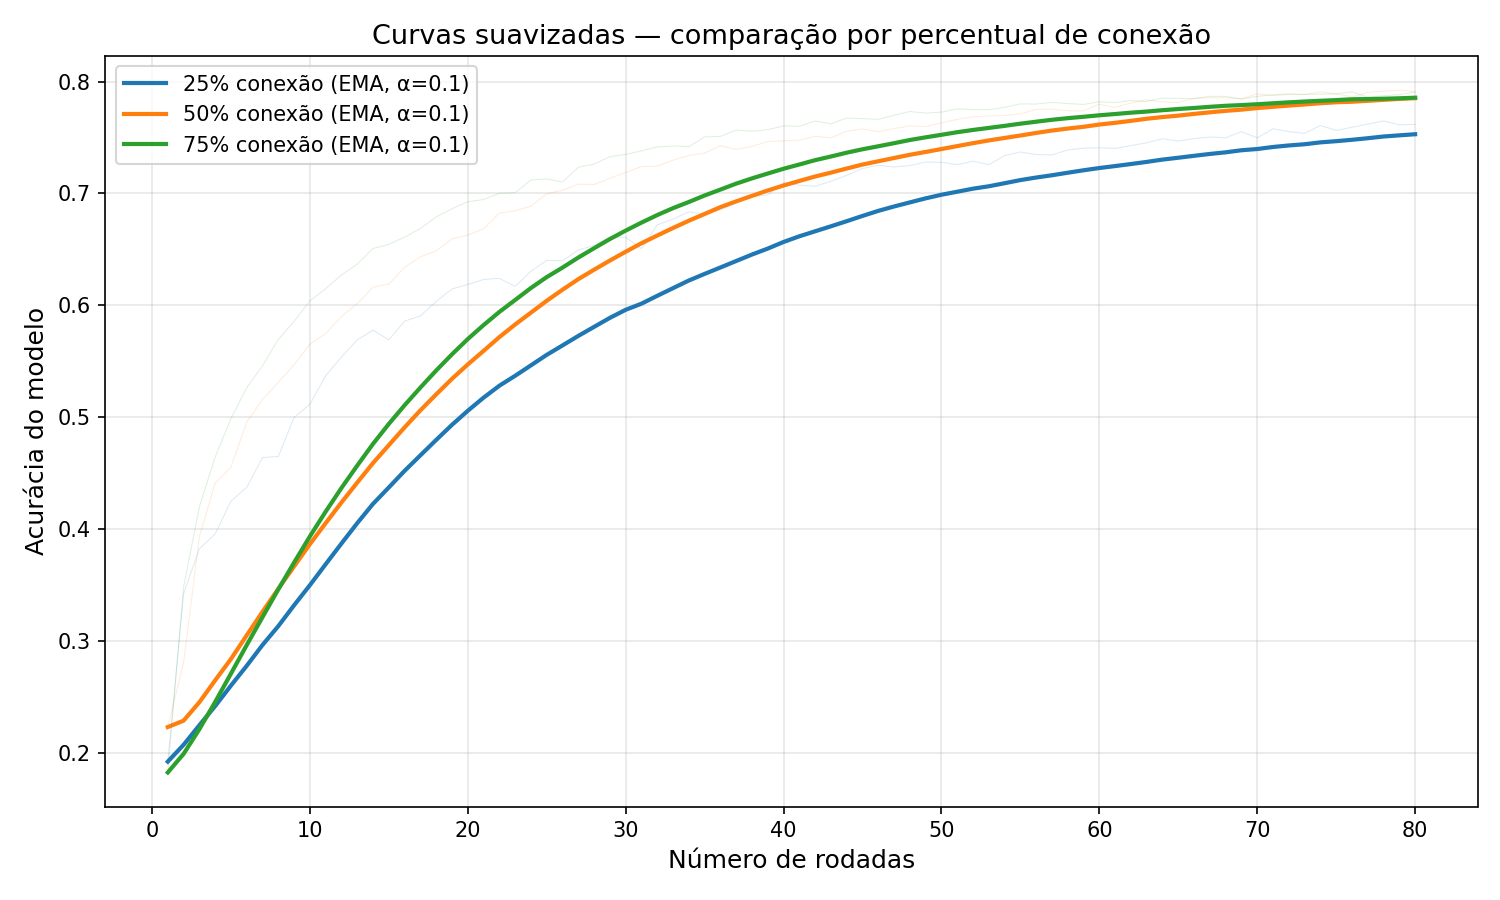
\includegraphics[width=\textwidth]{../synchronous/output-cifar-10/accuracy_iid.png}
    \caption{Síncrono / IID — curvas de acurácia suavizadas por EMA ($\alpha=0{,}1$), comparadas por percentual mínimo de conexão.}
\end{figure}

\begin{figure}[H]
    \centering
    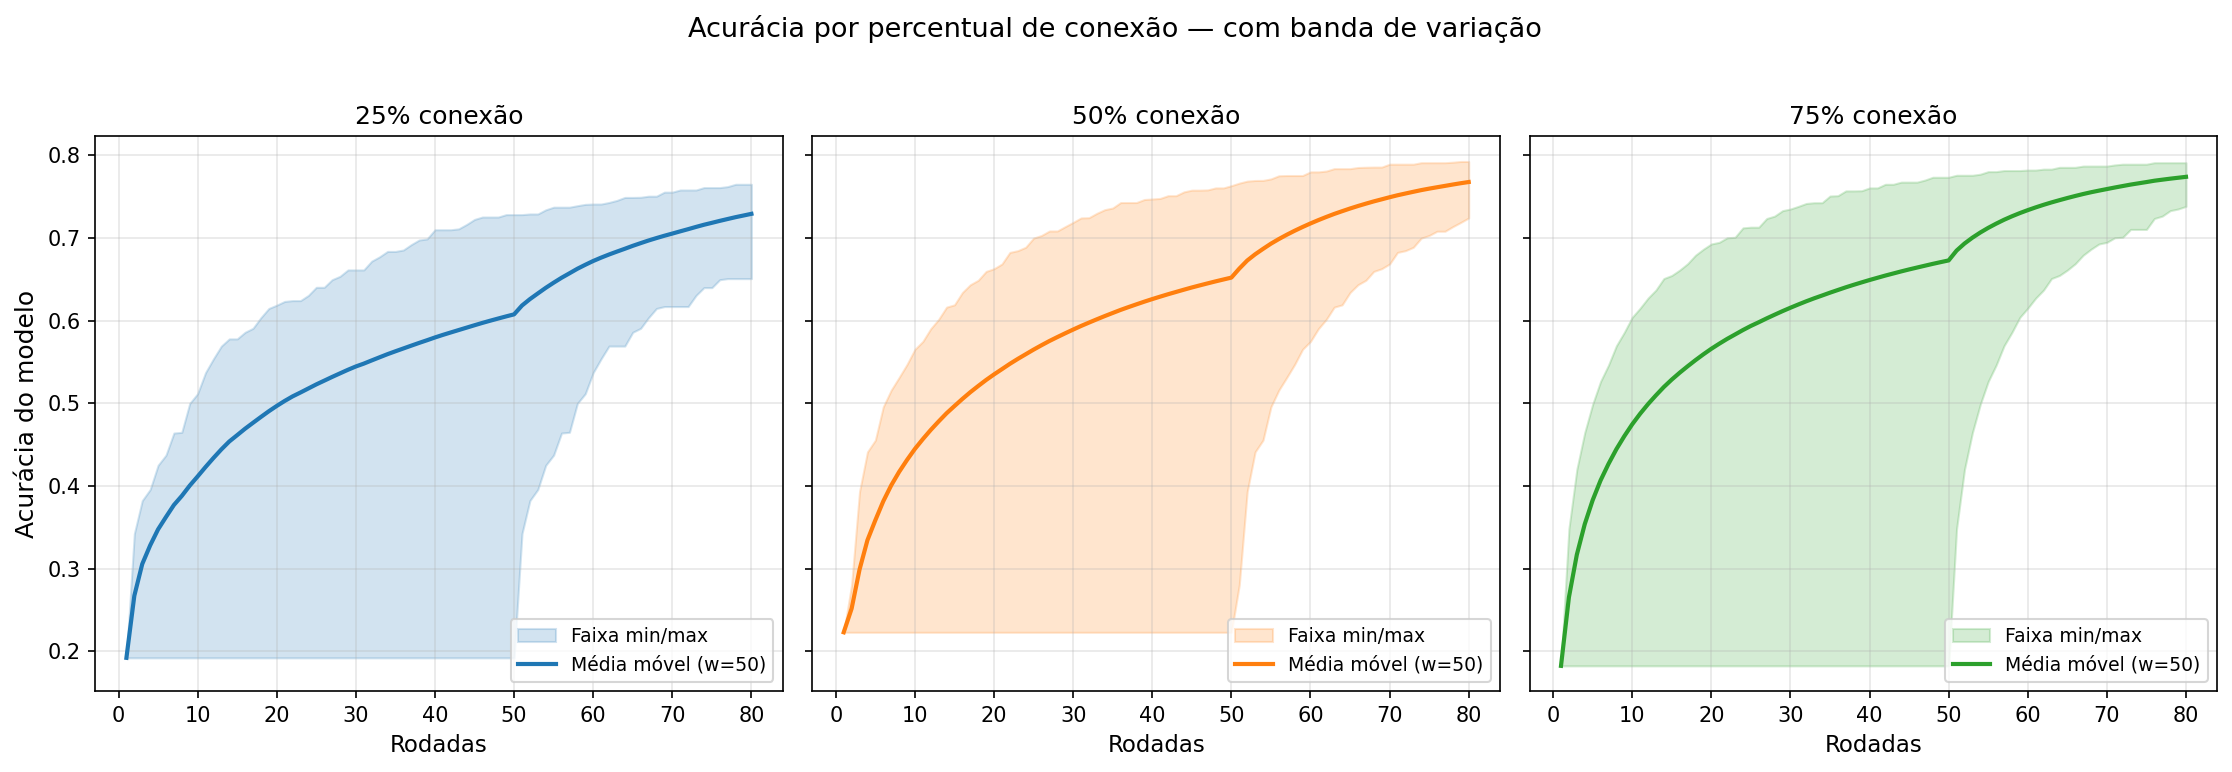
\includegraphics[width=\textwidth]{../synchronous/output-cifar-10/accuracy_bands_iid.png}
    \caption{Síncrono / IID — banda de confiança baseada no desvio absoluto suavizado por EMA ($\alpha=0{,}1$).}
\end{figure}

\begin{figure}[H]
    \centering
    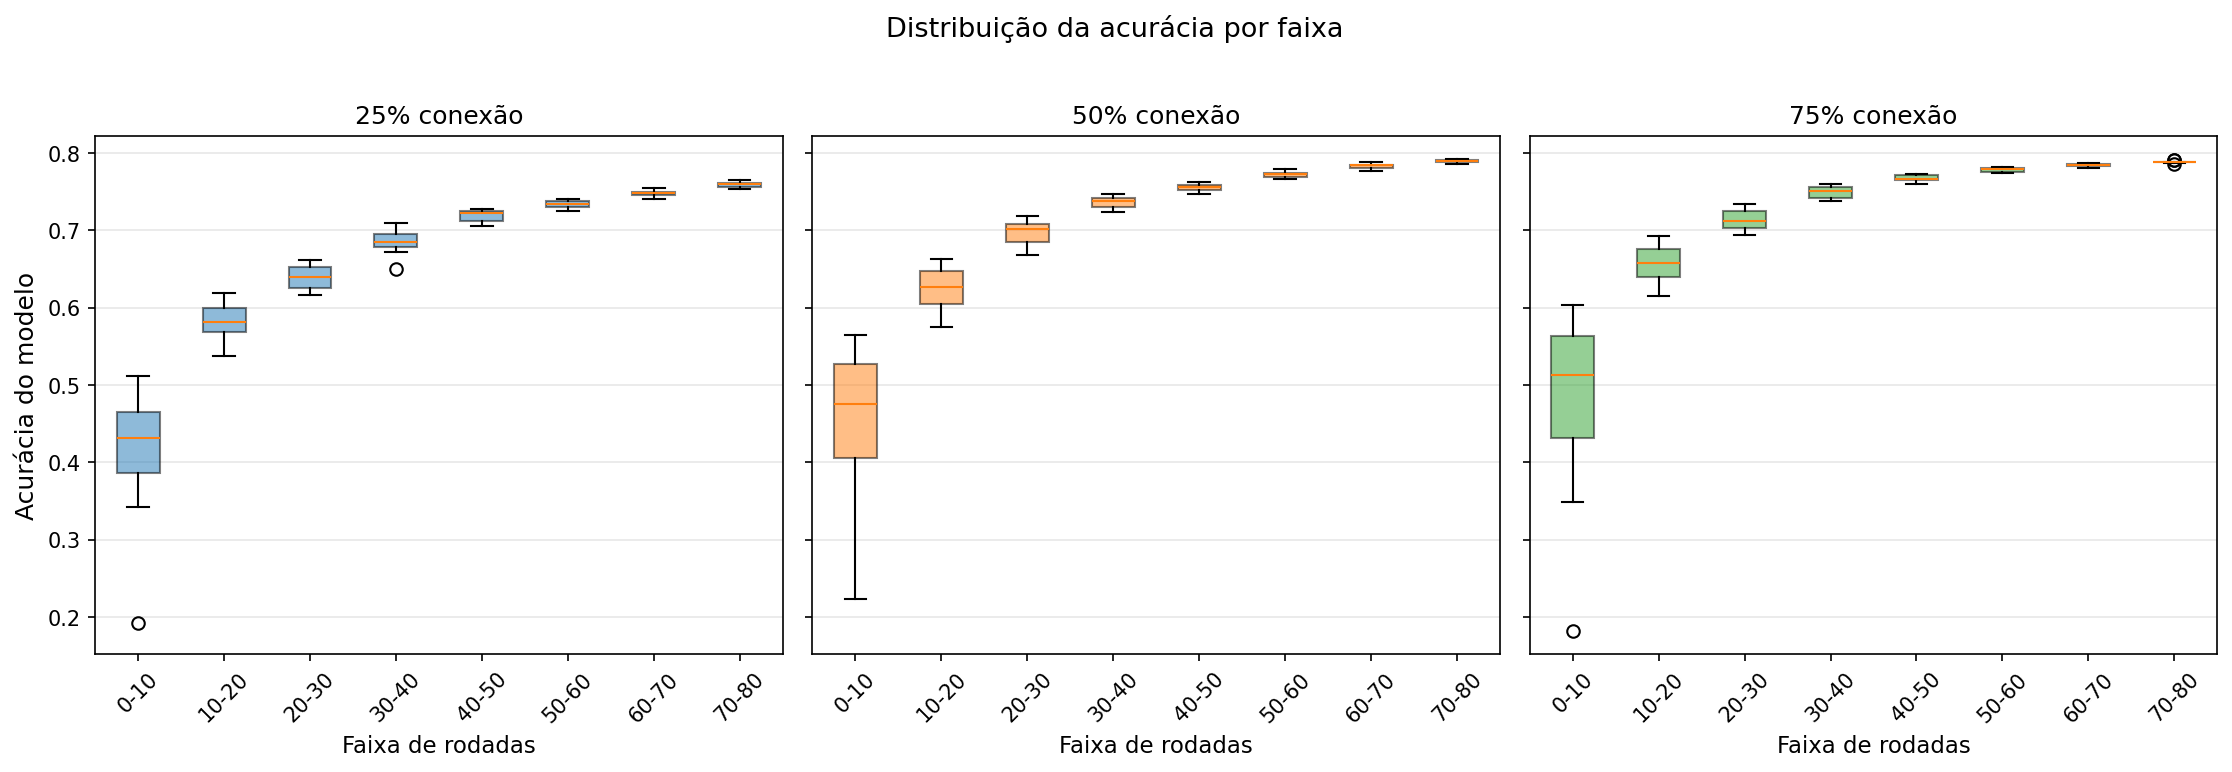
\includegraphics[width=\textwidth]{../synchronous/output-cifar-10/accuracy_boxplot_iid.png}
    \caption{Síncrono / IID — \textit{boxplot} por faixas de rodadas.}
\end{figure}

\subsection*{Não-IID}

\begin{figure}[H]
    \centering
    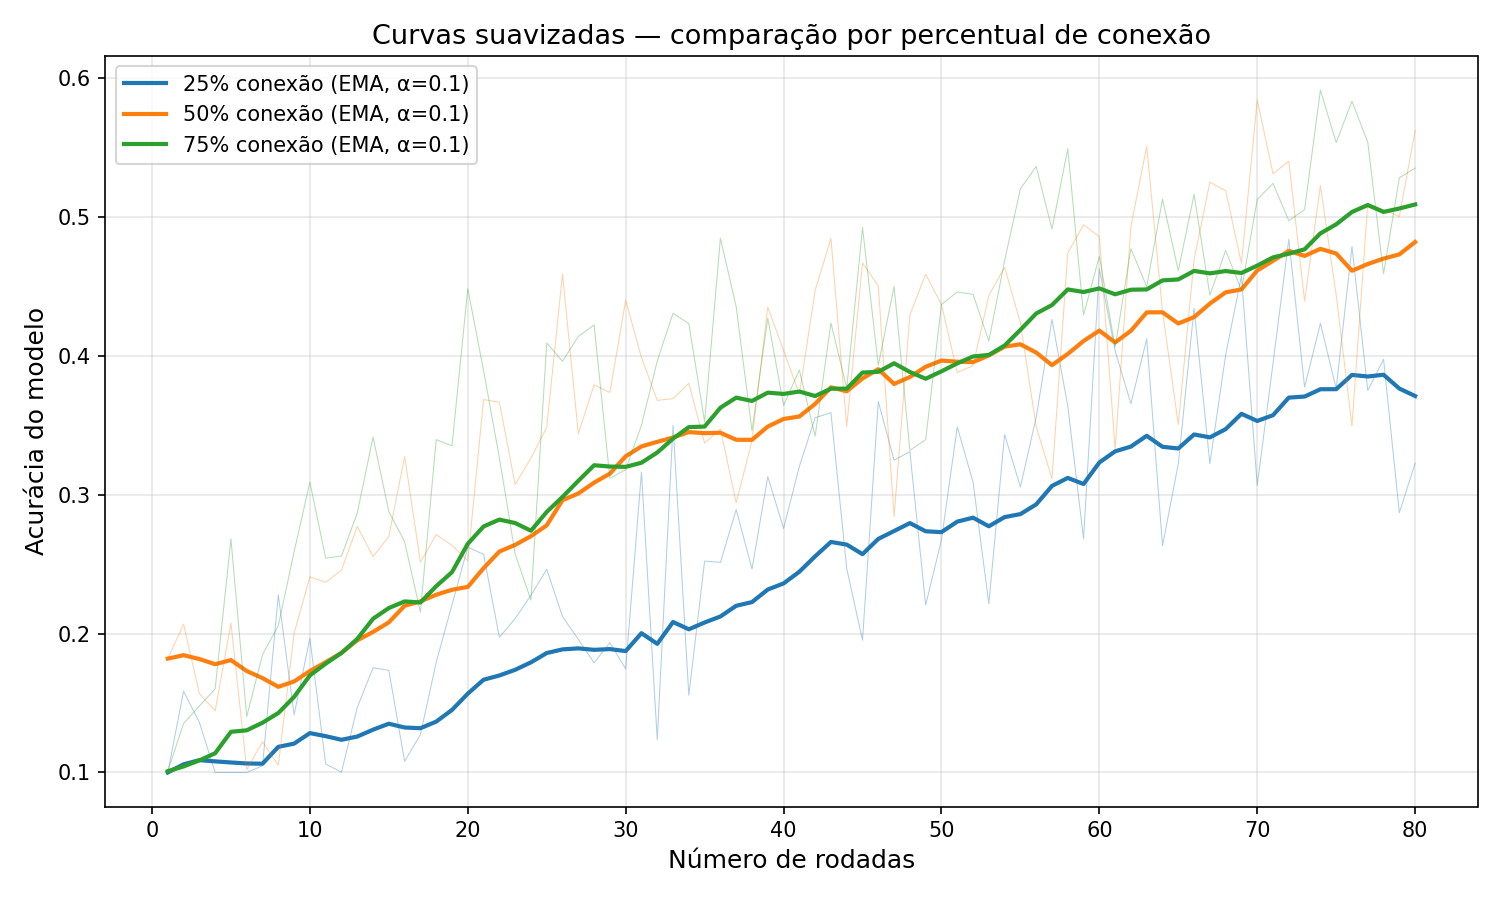
\includegraphics[width=\textwidth]{../synchronous/output-cifar-10/accuracy_non_iid.png}
    \caption{Síncrono / Não-IID — curvas de acurácia suavizadas por EMA ($\alpha=0{,}1$), comparadas por percentual mínimo de conexão.}
\end{figure}

\begin{figure}[H]
    \centering
    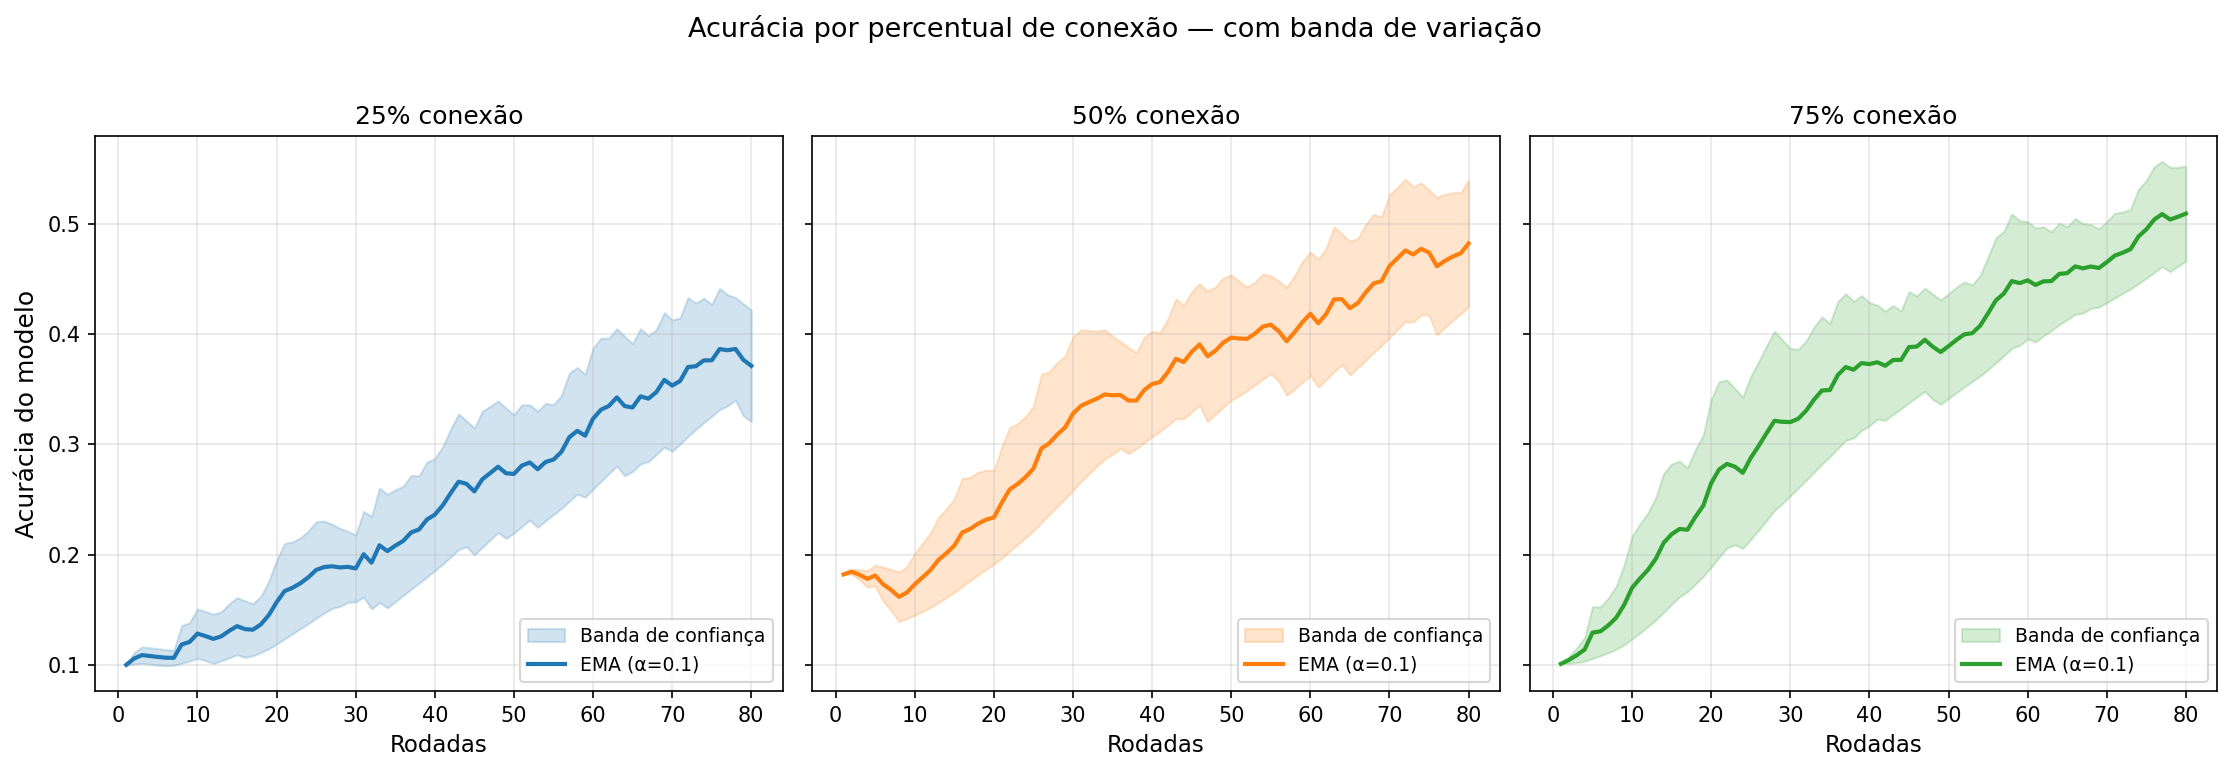
\includegraphics[width=\textwidth]{../synchronous/output-cifar-10/accuracy_bands_non_iid.png}
    \caption{Síncrono / Não-IID — banda de confiança baseada no desvio absoluto suavizado por EMA ($\alpha=0{,}1$).}
\end{figure}

\begin{figure}[H]
    \centering
    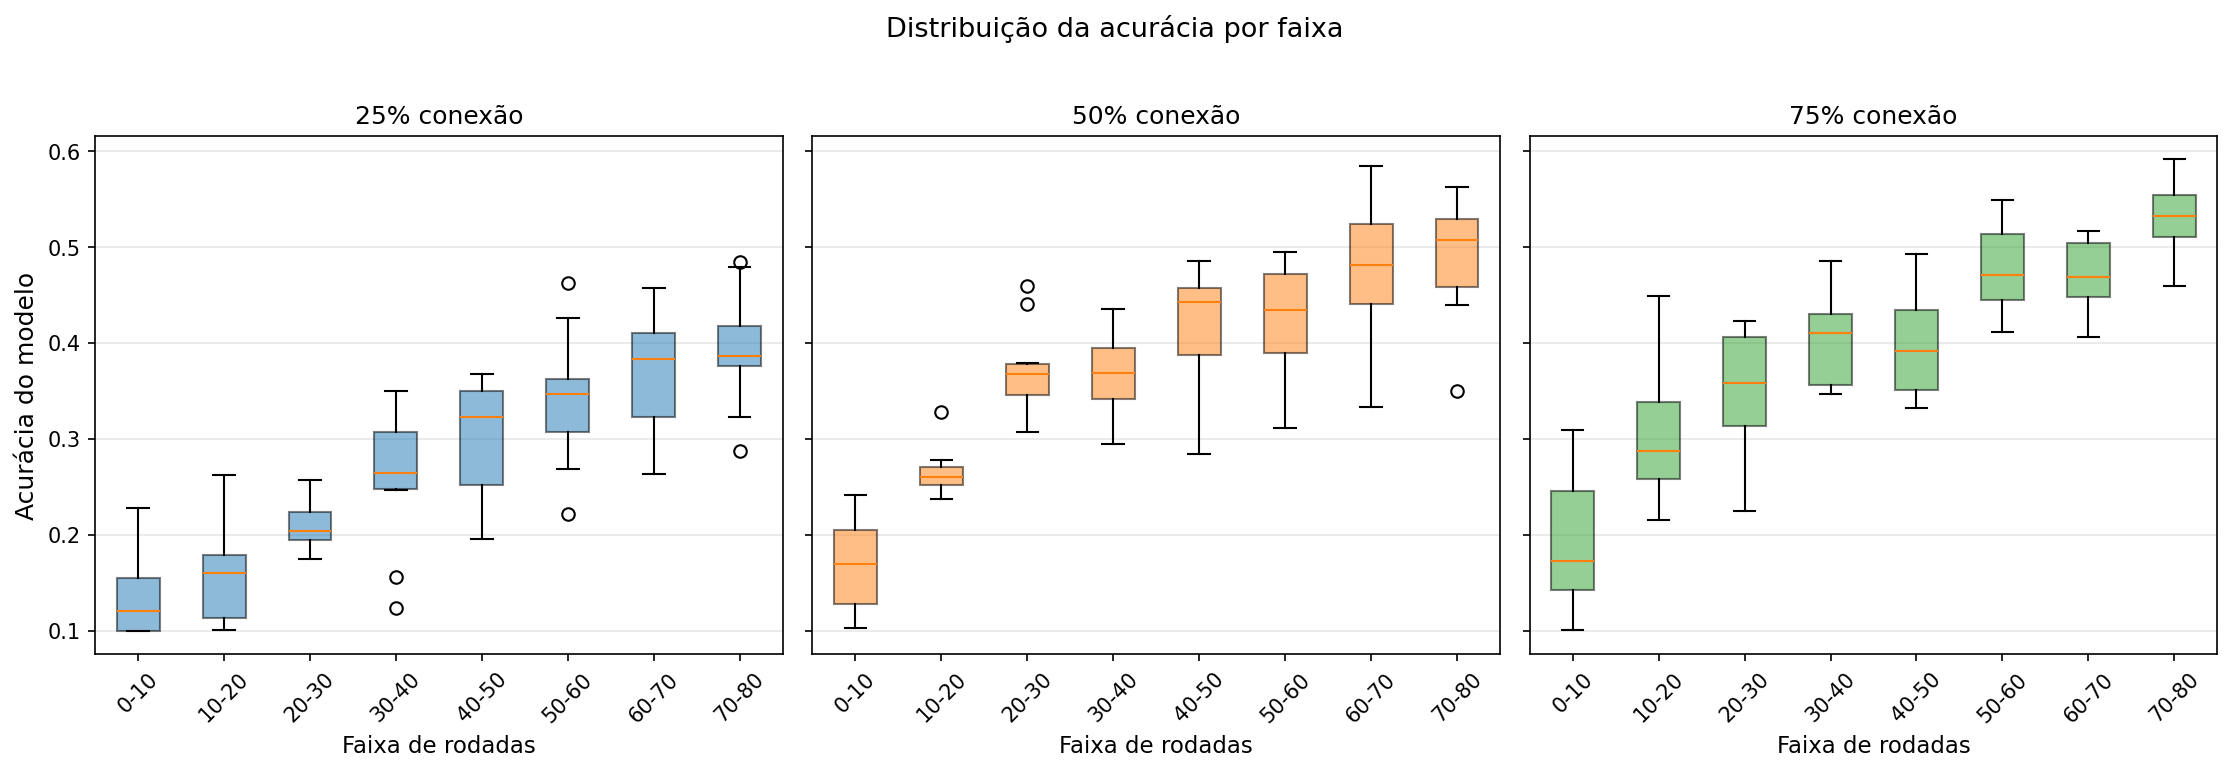
\includegraphics[width=\textwidth]{../synchronous/output-cifar-10/accuracy_boxplot_non_iid.png}
    \caption{Síncrono / Não-IID — \textit{boxplot} por faixas de rodadas.}
\end{figure}

% ─────────────────────────────────────────────
\section{Resultados — Assíncrono}

\subsection*{IID}

\begin{figure}[H]
    \centering
    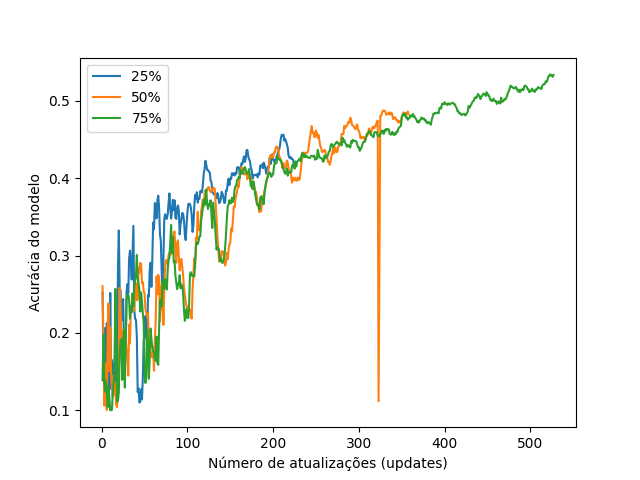
\includegraphics[width=\textwidth]{../asynchronous/output-cifar-10/accuracy_iid.png}
    \caption{Assíncrono / IID — curvas de acurácia suavizadas por EMA ($\alpha=0{,}1$), comparadas por \textit{timeout}.}
\end{figure}

\begin{figure}[H]
    \centering
    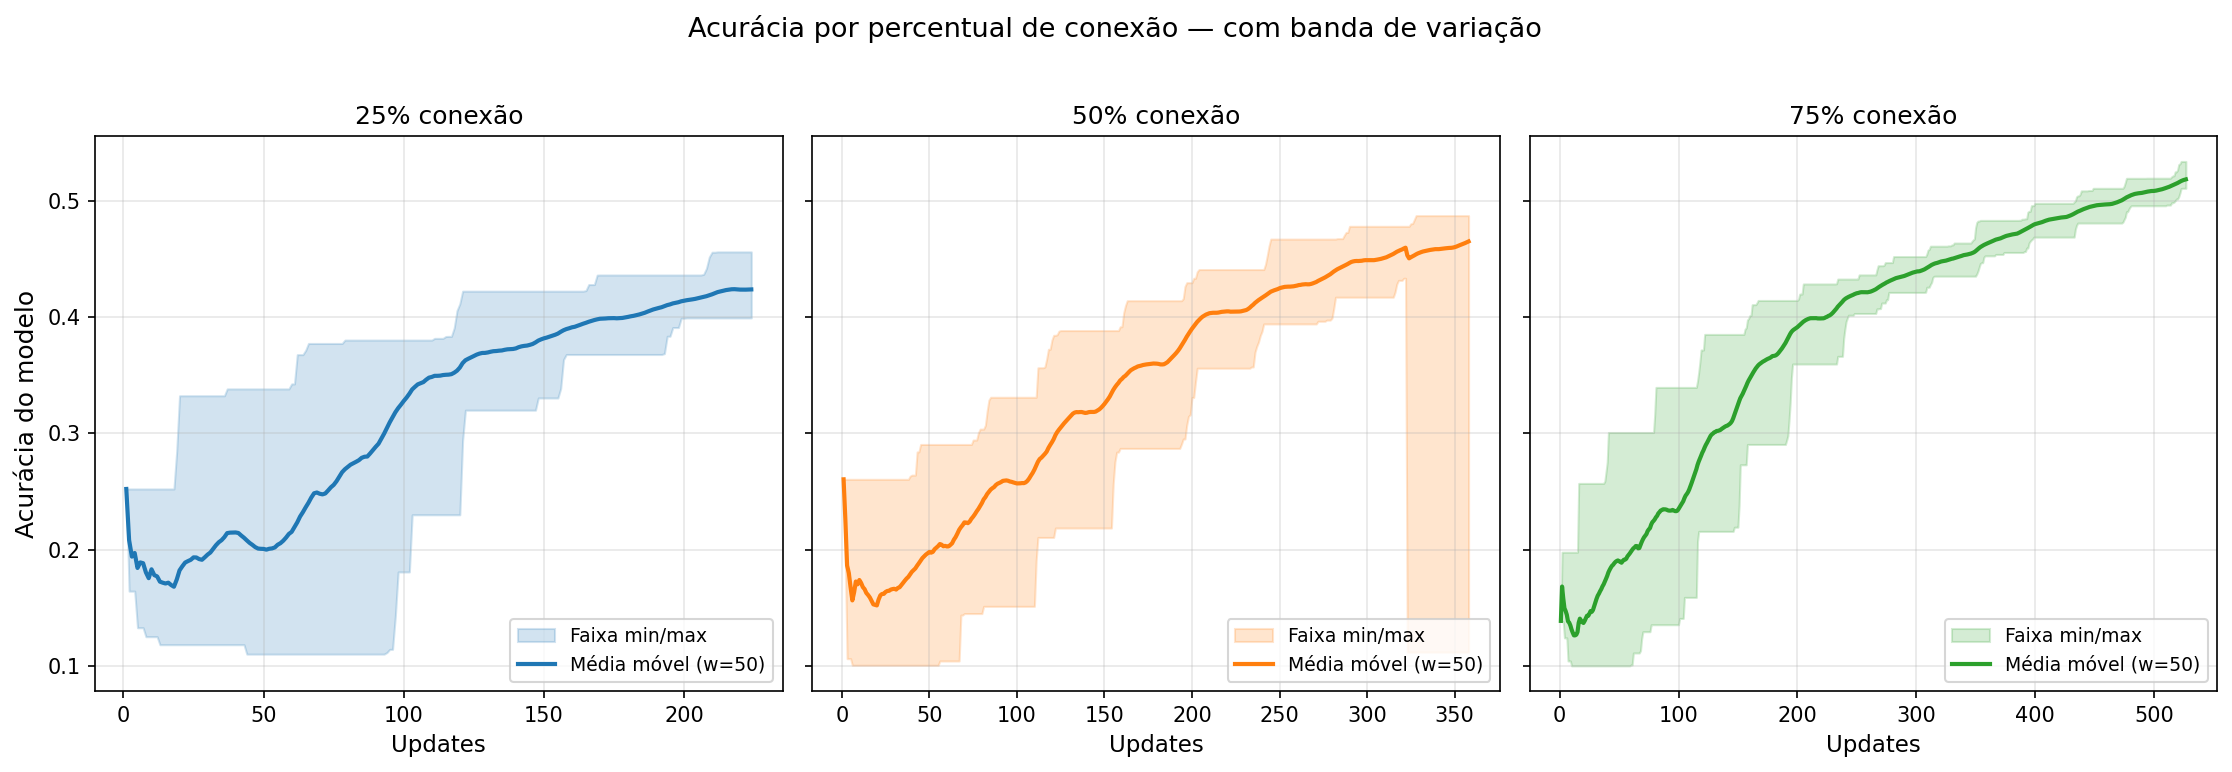
\includegraphics[width=\textwidth]{../asynchronous/output-cifar-10/accuracy_bands_iid.png}
    \caption{Assíncrono / IID — banda de confiança baseada no desvio absoluto suavizado por EMA ($\alpha=0{,}1$).}
\end{figure}

\begin{figure}[H]
    \centering
    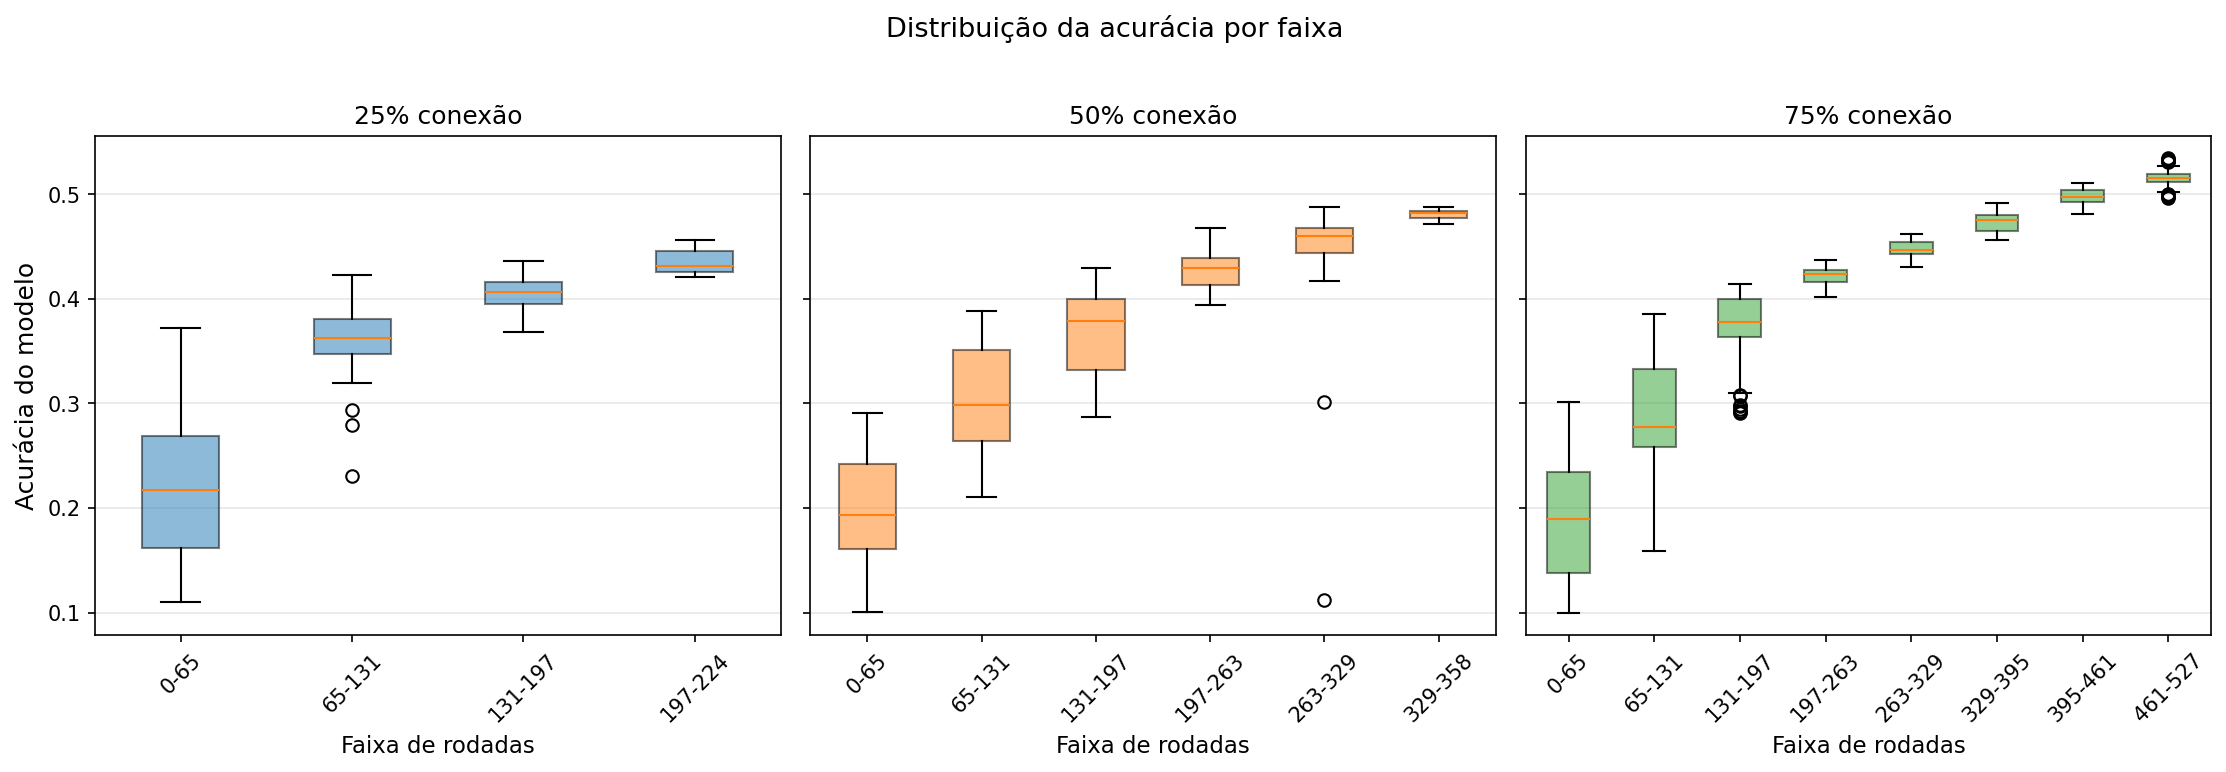
\includegraphics[width=\textwidth]{../asynchronous/output-cifar-10/accuracy_boxplot_iid.png}
    \caption{Assíncrono / IID — \textit{boxplot} por faixas de atualizações.}
\end{figure}

\subsection*{Não-IID}

\begin{figure}[H]
    \centering
    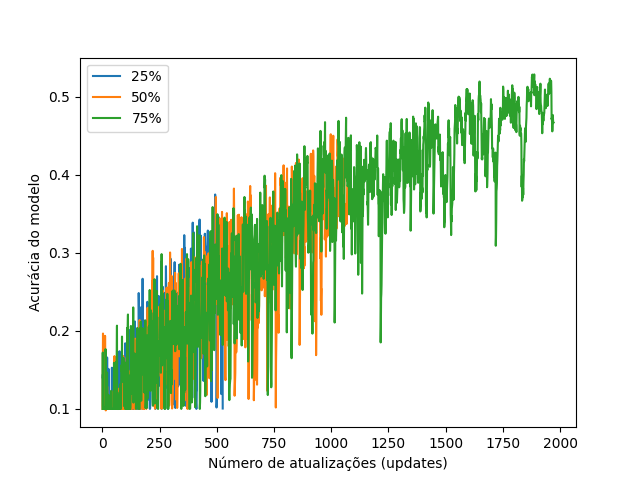
\includegraphics[width=\textwidth]{../asynchronous/output-cifar-10/accuracy_non_iid.png}
    \caption{Assíncrono / Não-IID — curvas de acurácia suavizadas por EMA ($\alpha=0{,}1$), comparadas por \textit{timeout}.}
\end{figure}

\begin{figure}[H]
    \centering
    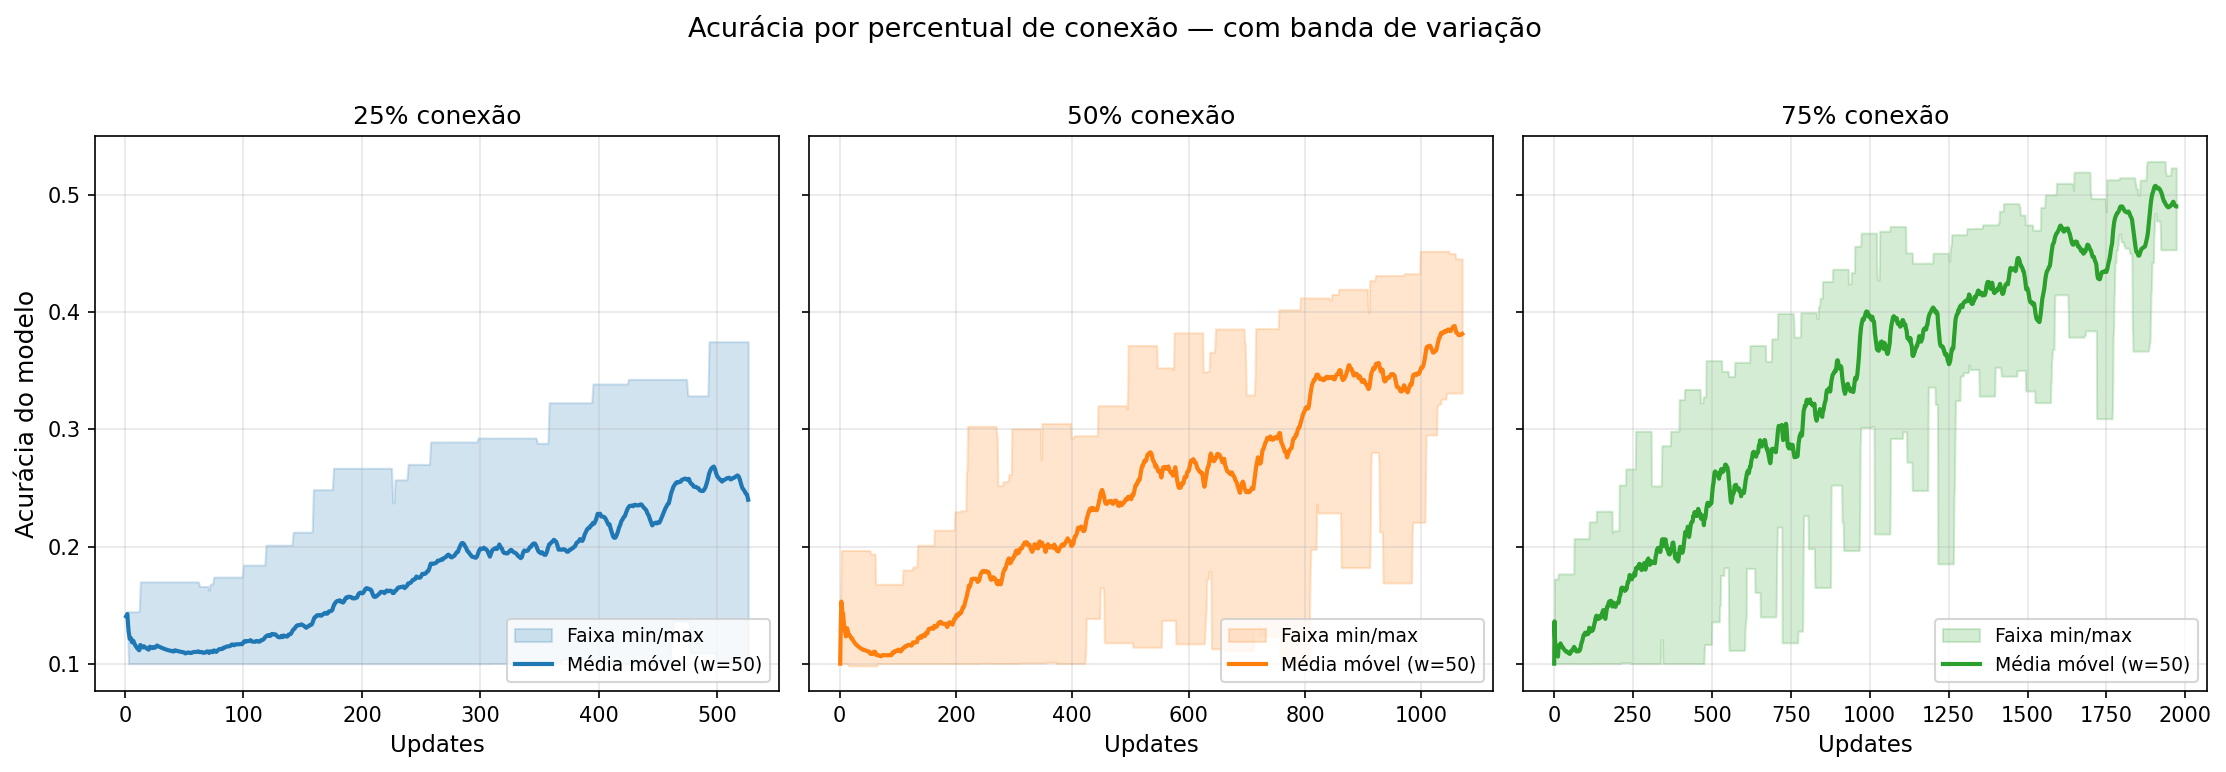
\includegraphics[width=\textwidth]{../asynchronous/output-cifar-10/accuracy_bands_non_iid.png}
    \caption{Assíncrono / Não-IID — banda de confiança baseada no desvio absoluto suavizado por EMA ($\alpha=0{,}1$).}
\end{figure}

\begin{figure}[H]
    \centering
    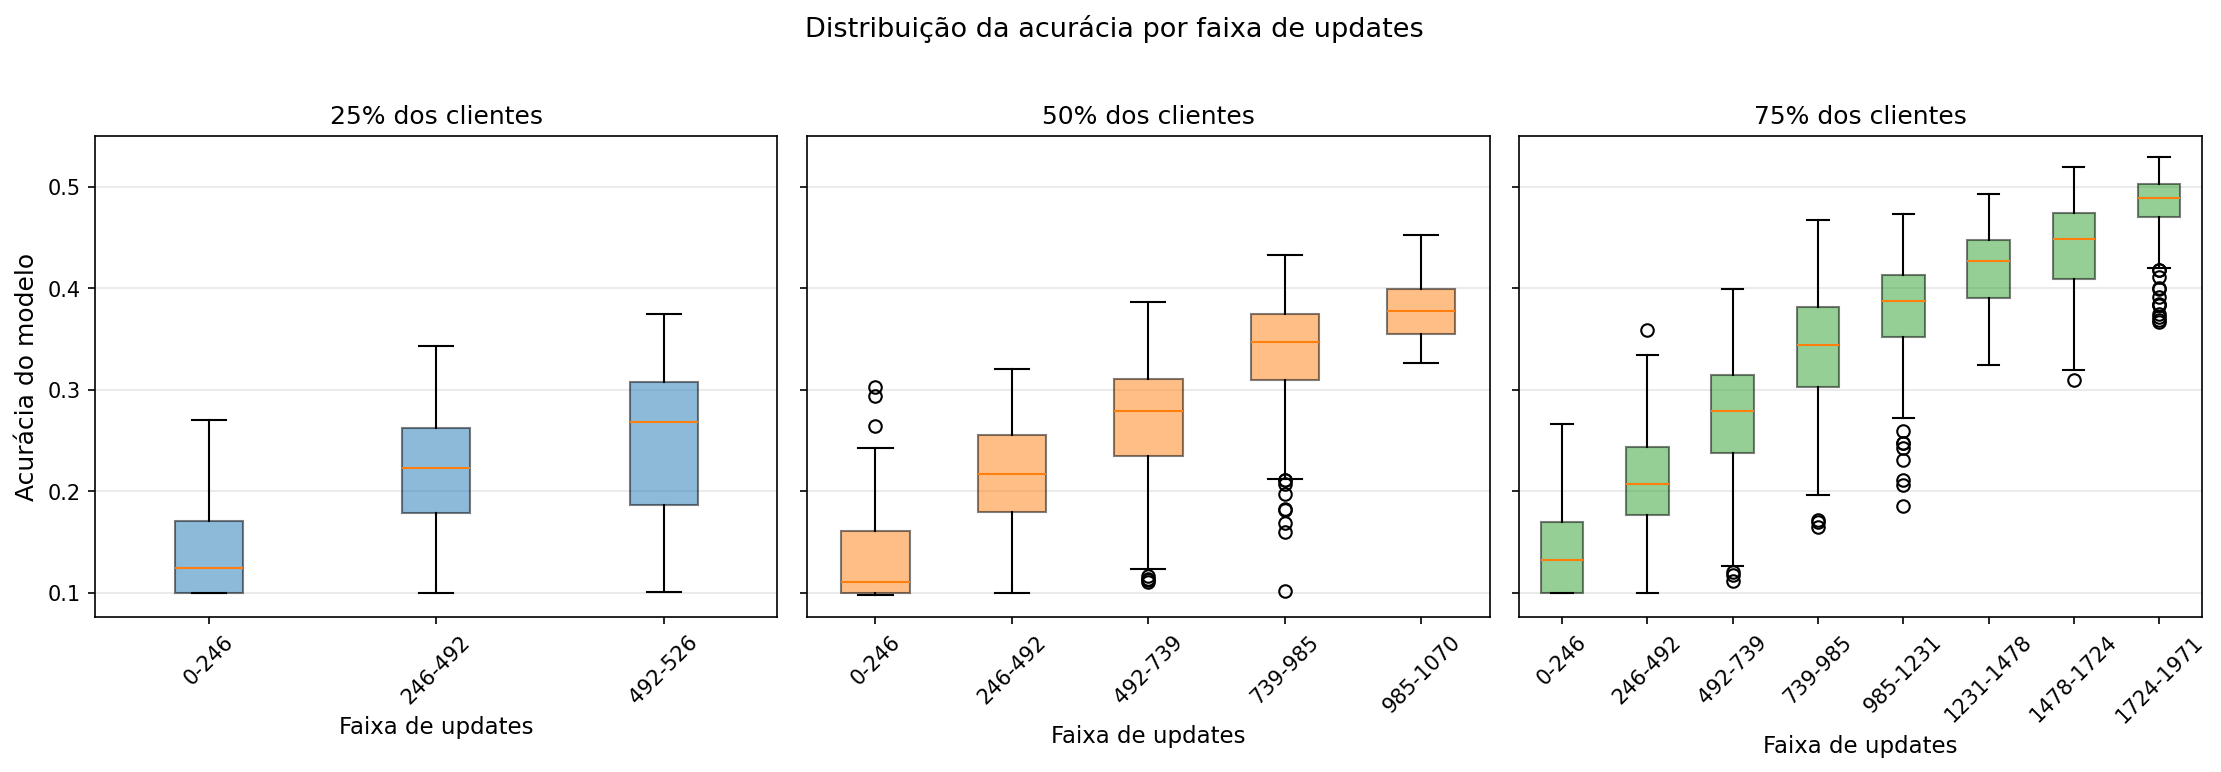
\includegraphics[width=\textwidth]{../asynchronous/output-cifar-10/accuracy_boxplot_non_iid.png}
    \caption{Assíncrono / Não-IID — \textit{boxplot} por faixas de atualizações.}
\end{figure}

\end{document}